\documentclass[12pt,aspectratio=1610]{beamer}
\usetheme{Copenhagen}
\usecolortheme{seahorse}
\usepackage{amsmath,amssymb,mathtools}
\usepackage{caption}
\usepackage{subcaption}
\setbeamertemplate{footline}{}
\setbeamertemplate{navigation symbols}{}

\title{Modulation Instability in Semiconductor Quantum Dots}
\subtitle{Y-type Excitation Scheme}
\author{Shaon Samanta\\
        Department of Physics (MSc.)\\
        Sem-IV\\[1.2em]
        \textit{Supervised by,}\\
        Dr.\ Rohit Mukherjee\\
        Assistant Professor of Dept.\ of Physics (MSc.)\\
        Sarala Birla University}
\date{}

\begin{document}

\frame{\titlepage}

\begin{frame}{Overview}
  \vspace{-3pt}
  \begin{itemize}
    \item Motivation: Understanding Modulation Instability (MI) in SQDs (Y-type excitation).
    \item Tools: Density matrix formalism, NLSE\@.
    \item Focus: Interpretation of numerical plots \& physical insights.
  \end{itemize}
\end{frame}

\begin{frame}{Light Matter Interaction}
  \vspace{-20pt}
  \hspace*{55pt}
  \begin{figure}
    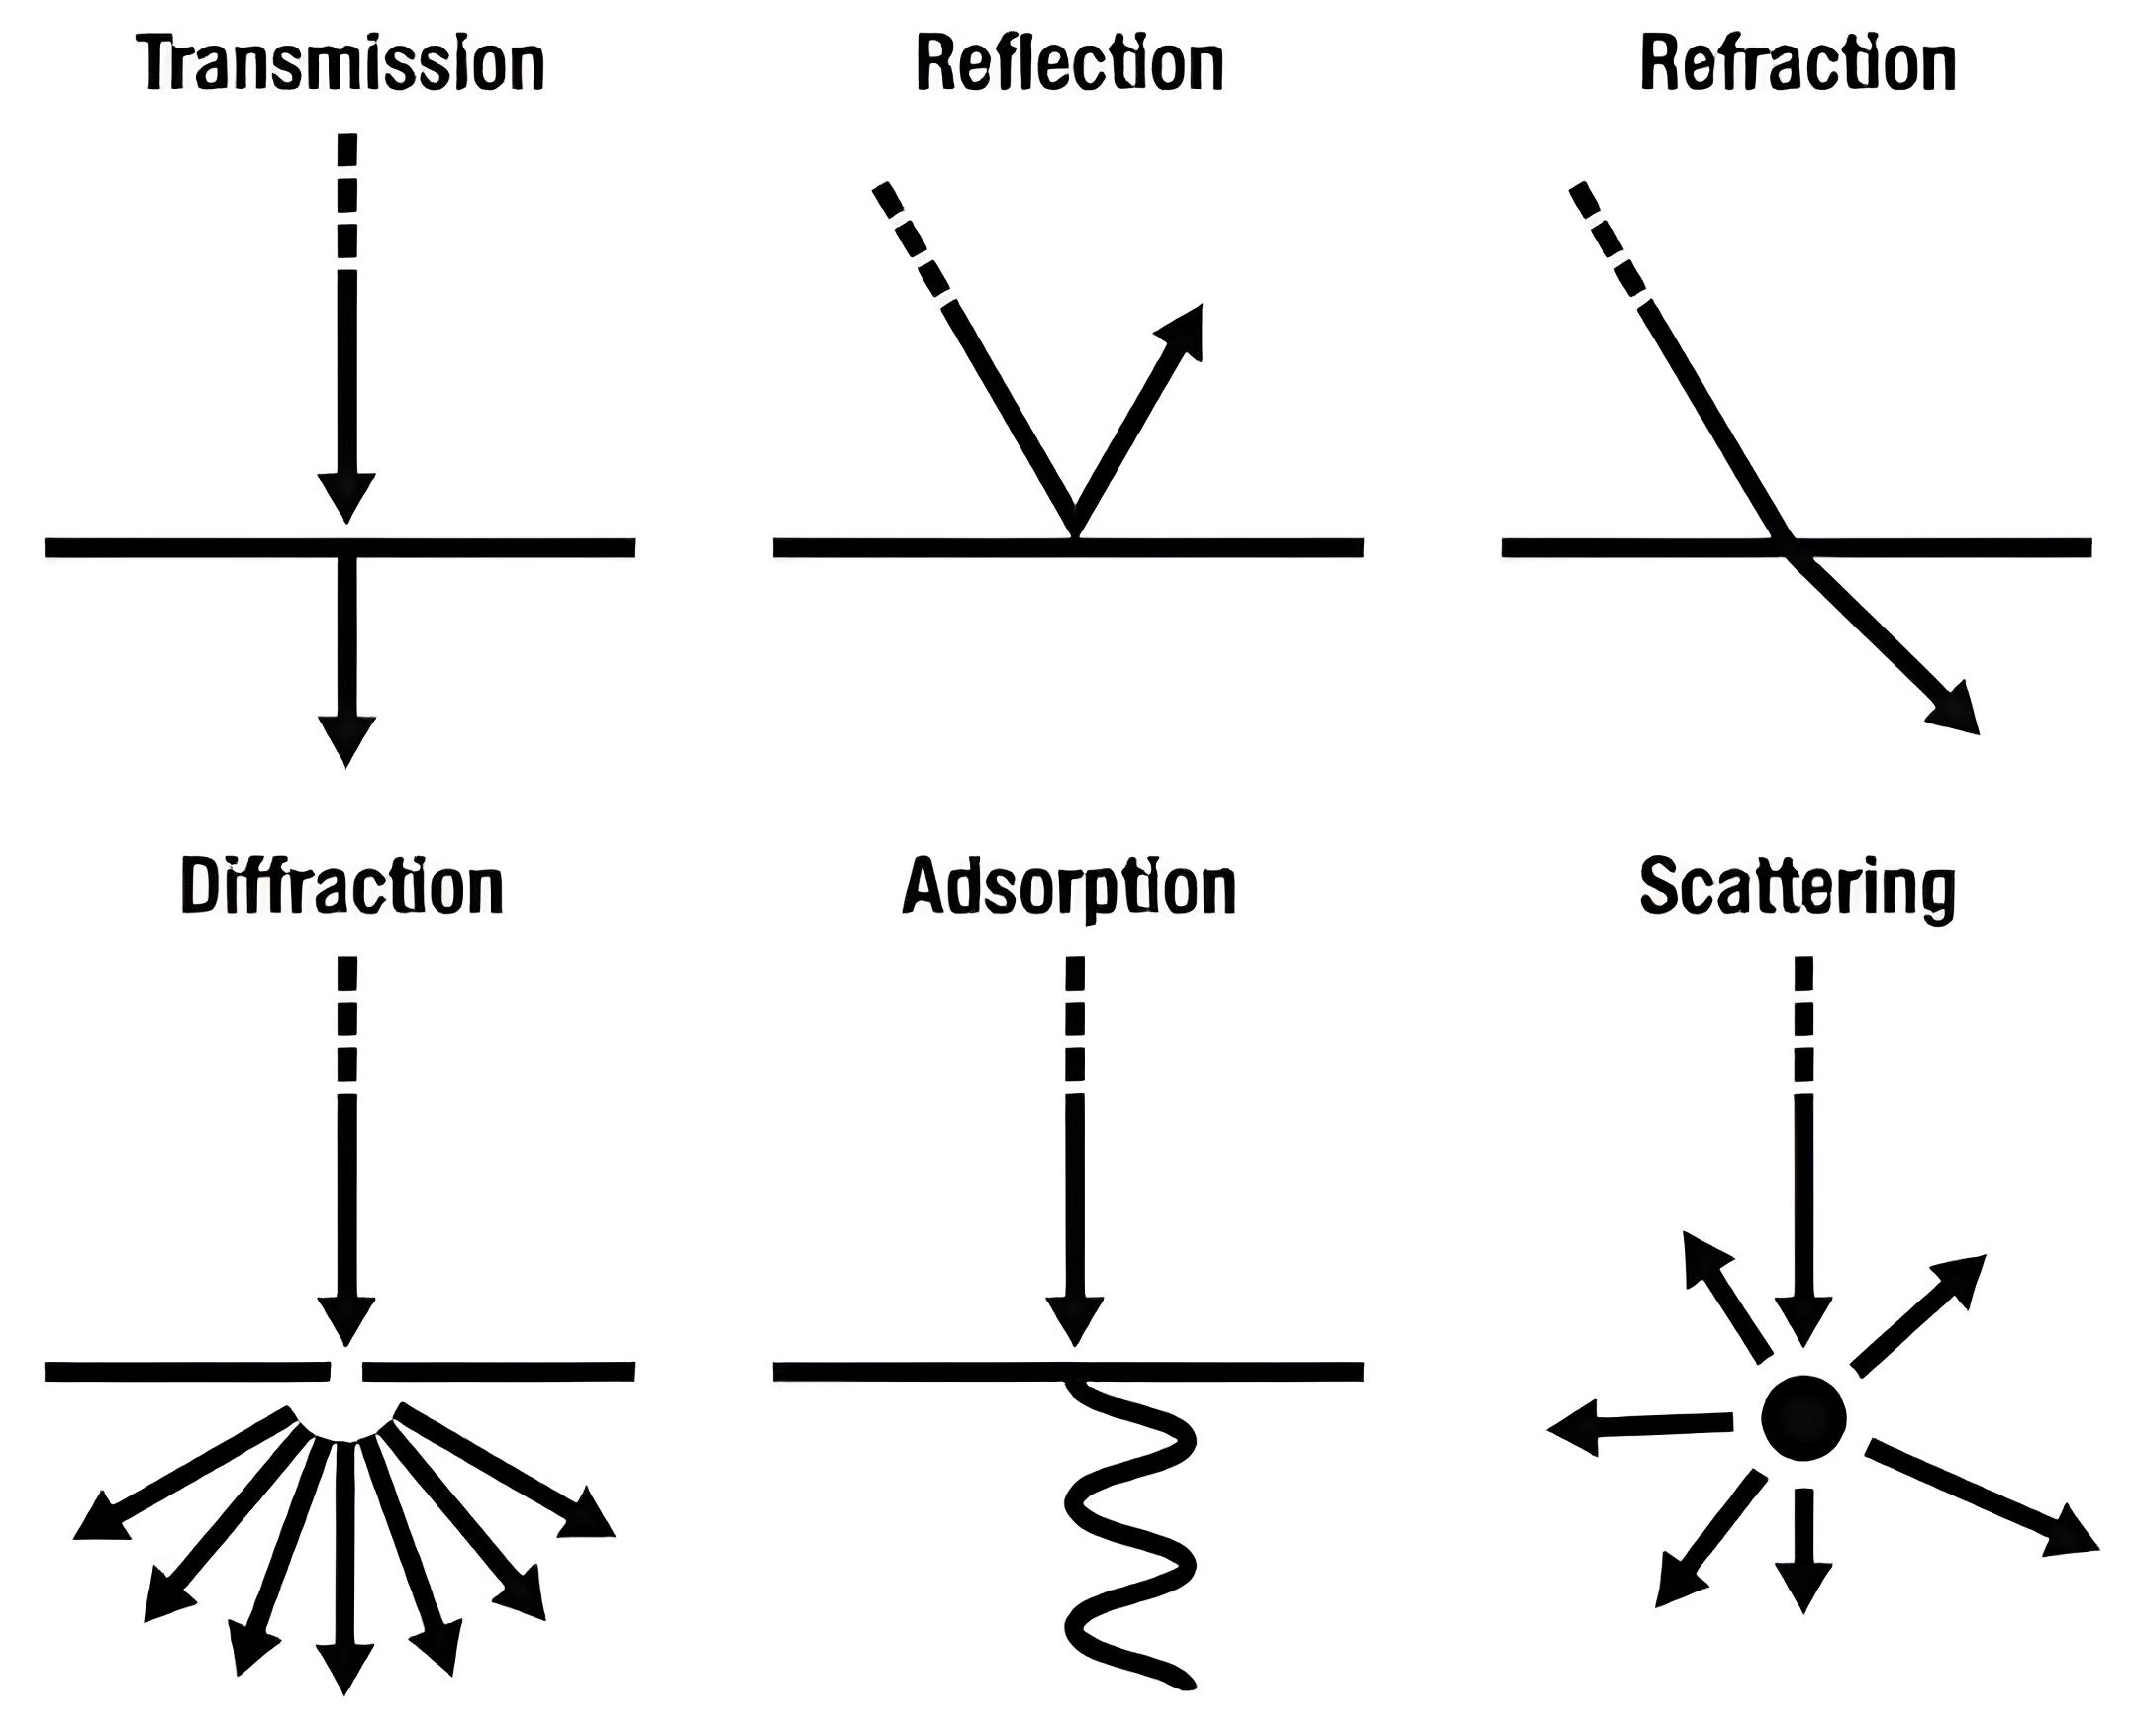
\includegraphics[width=0.5\textwidth]{Assets/Light Matter Interaction.jpeg}
  \end{figure}
  \begin{itemize}
    \item Quantum dots confine charge carriers in all three dimensions.
    \item Enhanced interaction with electromagnetic fields due to confinement.
    \item Leads to strong nonlinear effects: Kerr nonlinearity, EIT, and MI\@.
  \end{itemize}
\end{frame}

\begin{frame}{What are Semiconductor Quantum Dots}
  \begin{itemize}
    \item Tiny semiconductor nanocrystals (2--10 nm in size).
    \item Exhibit size-dependent fluorescence, unique electronic properties, enhanced optical properties.
    \item Intermediate properties between bulk semiconductors and discrete molecules.
  \end{itemize}
  \vspace{15pt}
  \centering
  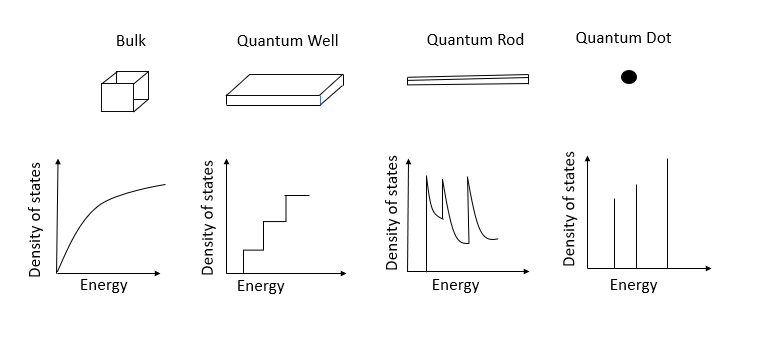
\includegraphics[width=0.75\textwidth]{Assets/DoSvsE.PNG}
\end{frame}

\begin{frame}{Y-type Excitation Scheme in SQDs}
  \vspace{-20pt}
  \begin{figure}
    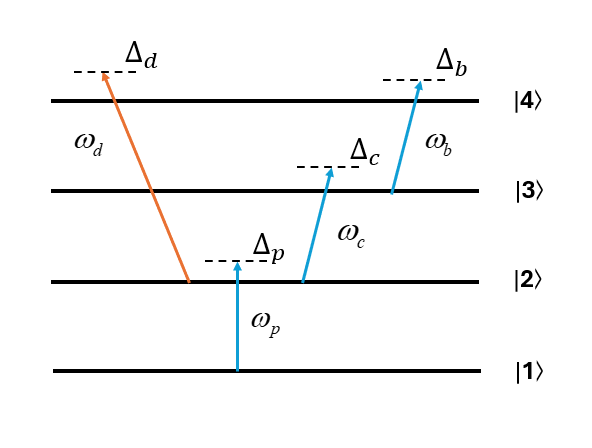
\includegraphics[width=0.6\textwidth]{Assets/Y-type.png}
  \end{figure}
  \vspace{-12pt}
  \begin{itemize}
    \item Probe field couples levels $|1\rangle \rightarrow |2\rangle$.
    \item Control fields modulate transitions $|2\rangle \rightarrow |3\rangle$, $|3\rangle \rightarrow |4\rangle$.
    \item The interacting electric field inside QD is: \( \vec{E}=\sum_{j=p,c,b}\hat{e}_j E_j e^{i(k_j z-\omega_j t)} \)
  \end{itemize}
\end{frame}

\begin{frame}{Modulation Instability}
  \begin{itemize}
    \item It is a process where a small perturbation on a Continuous Wave grows exponentially as it propagates through dispersive media.
    \item It happens due to interplay between nonlinear effects and dispersion.
    \item It produces the periodic wave train whose amplitude is high.
    \item It is a wave breaking process where stable wave become unstable and cause modulation instability
  \end{itemize}
\end{frame}

\begin{frame}{Absorption \& Dispersion Spectra}
  \vspace{-22pt}
  \begin{figure}[h]
    \centering
    \begin{minipage}{0.48\textwidth}
      \centering
      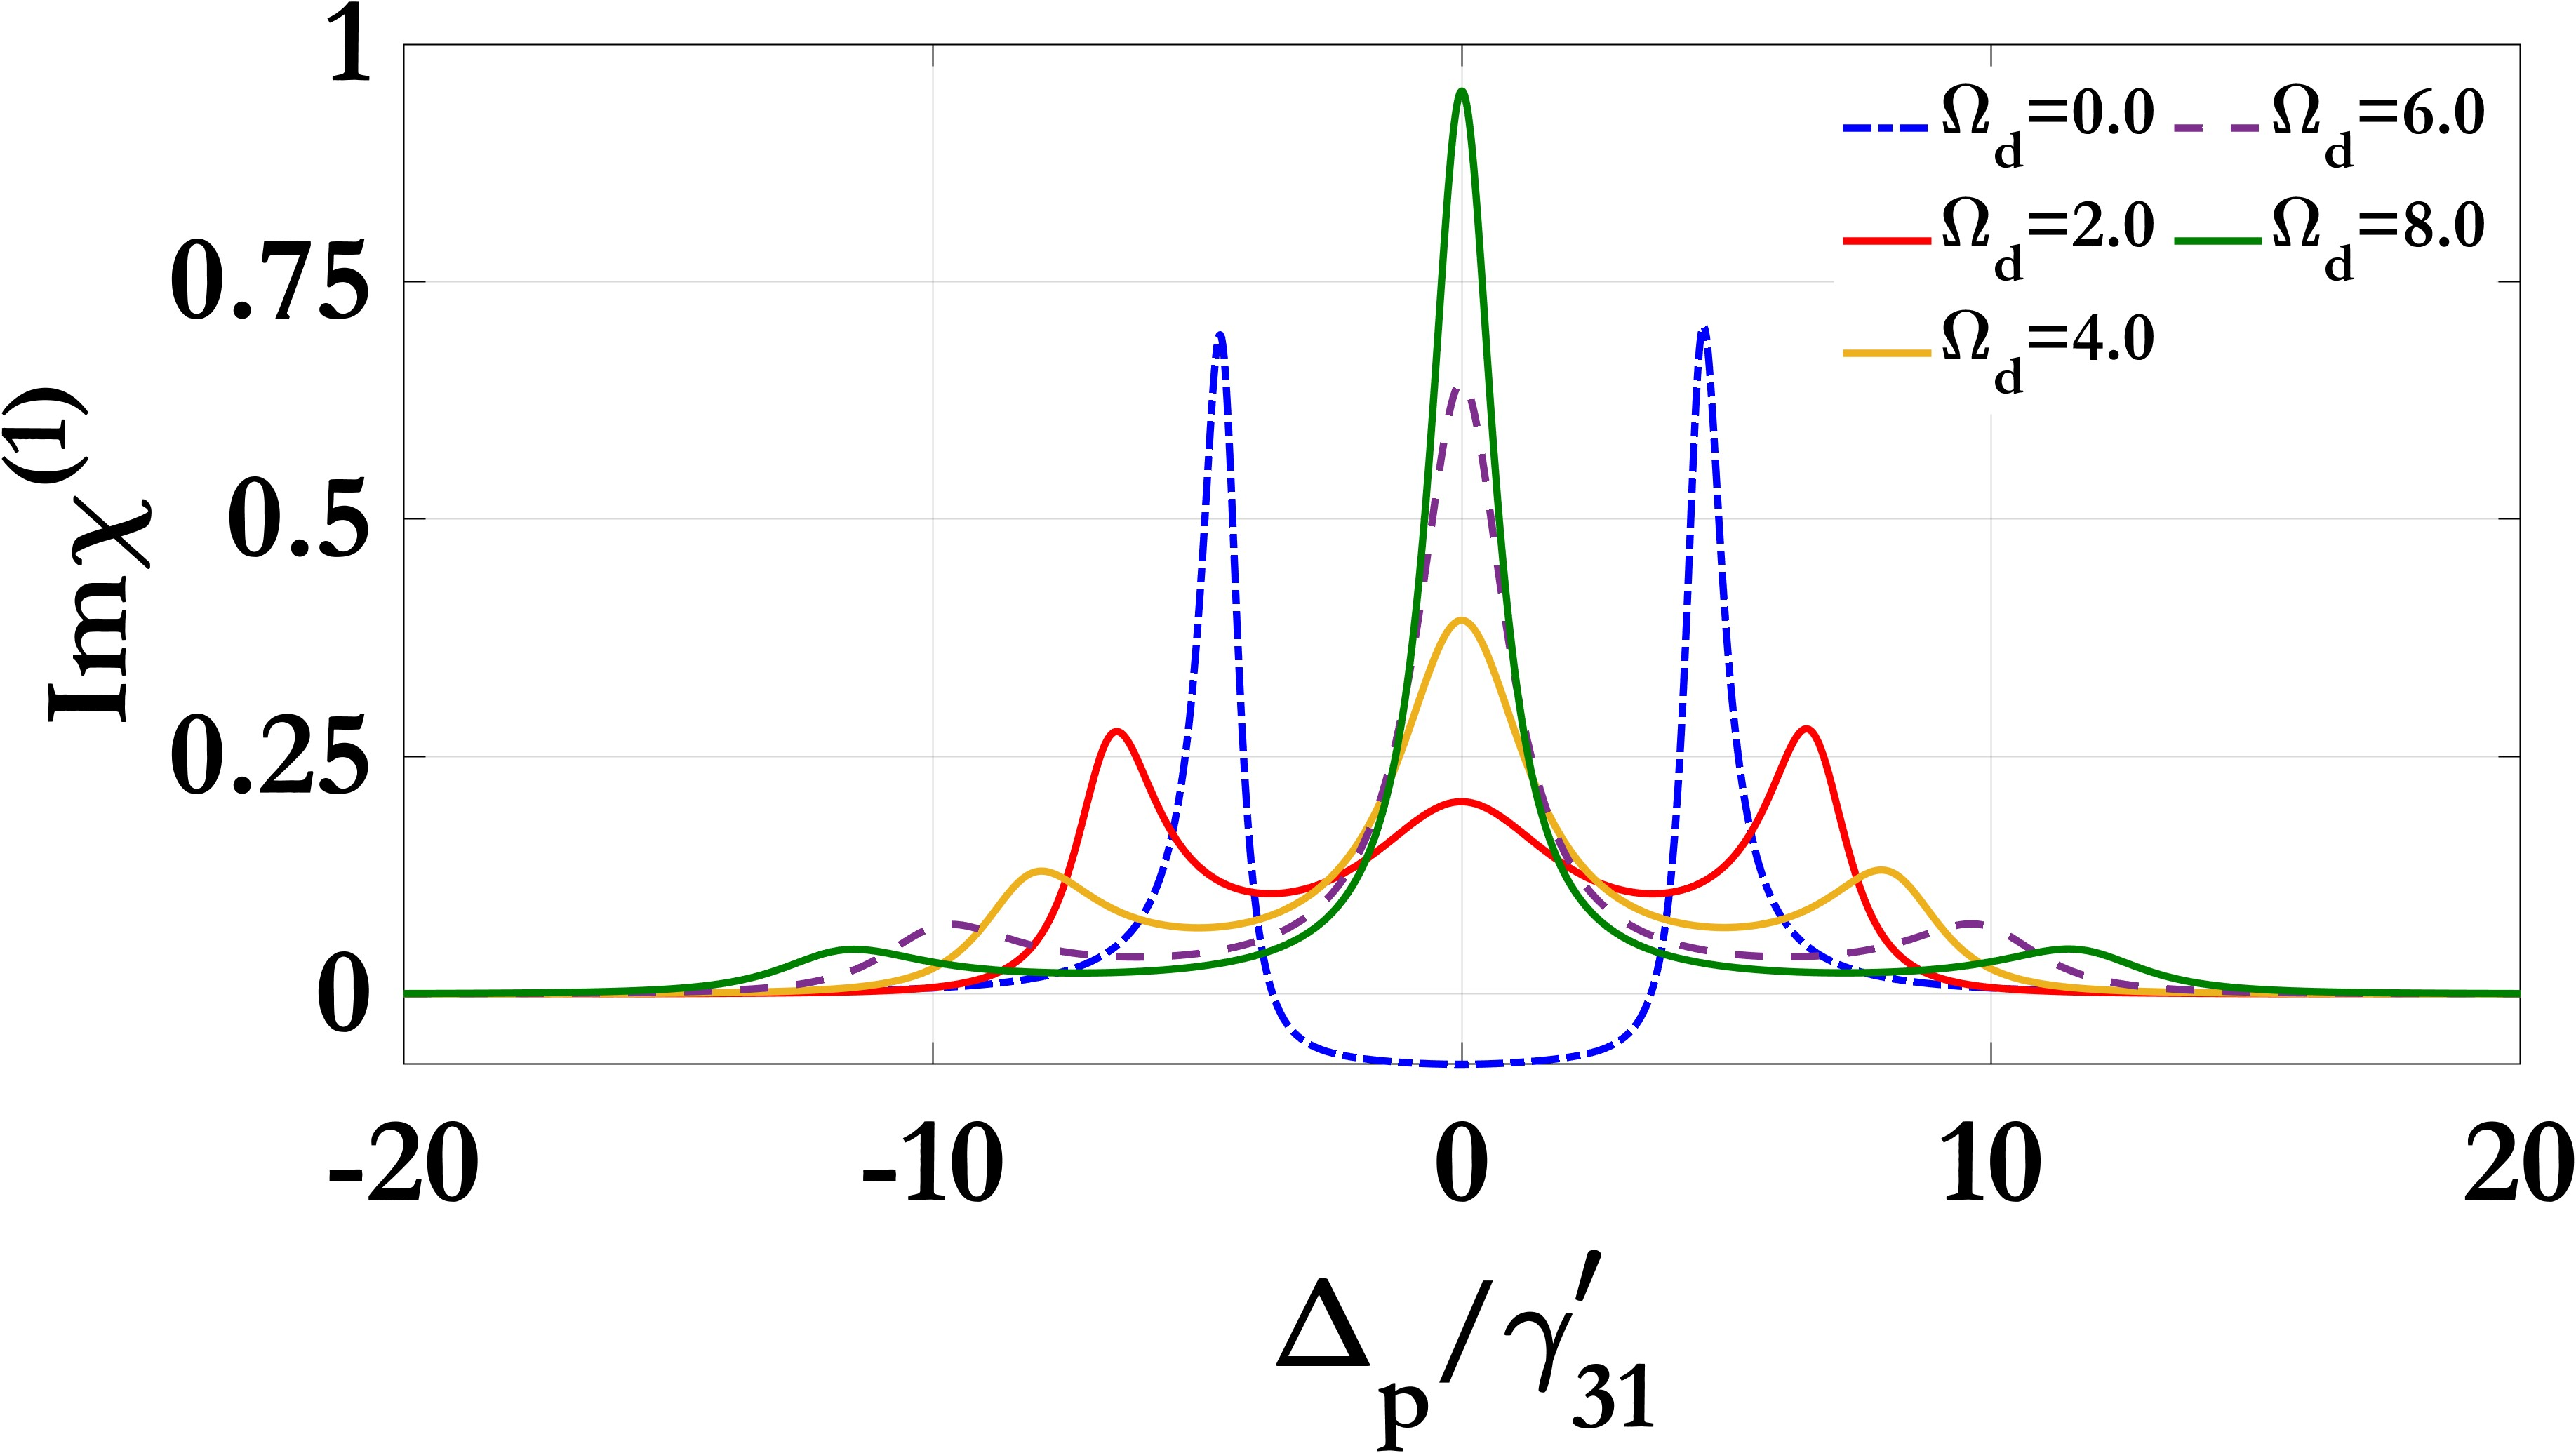
\includegraphics[width=\linewidth]{Assets/Img_chi1_Omega_d.jpeg}
      \subcaption{}
    \end{minipage}
    \hfill
    \begin{minipage}{0.48\textwidth}
      \centering
      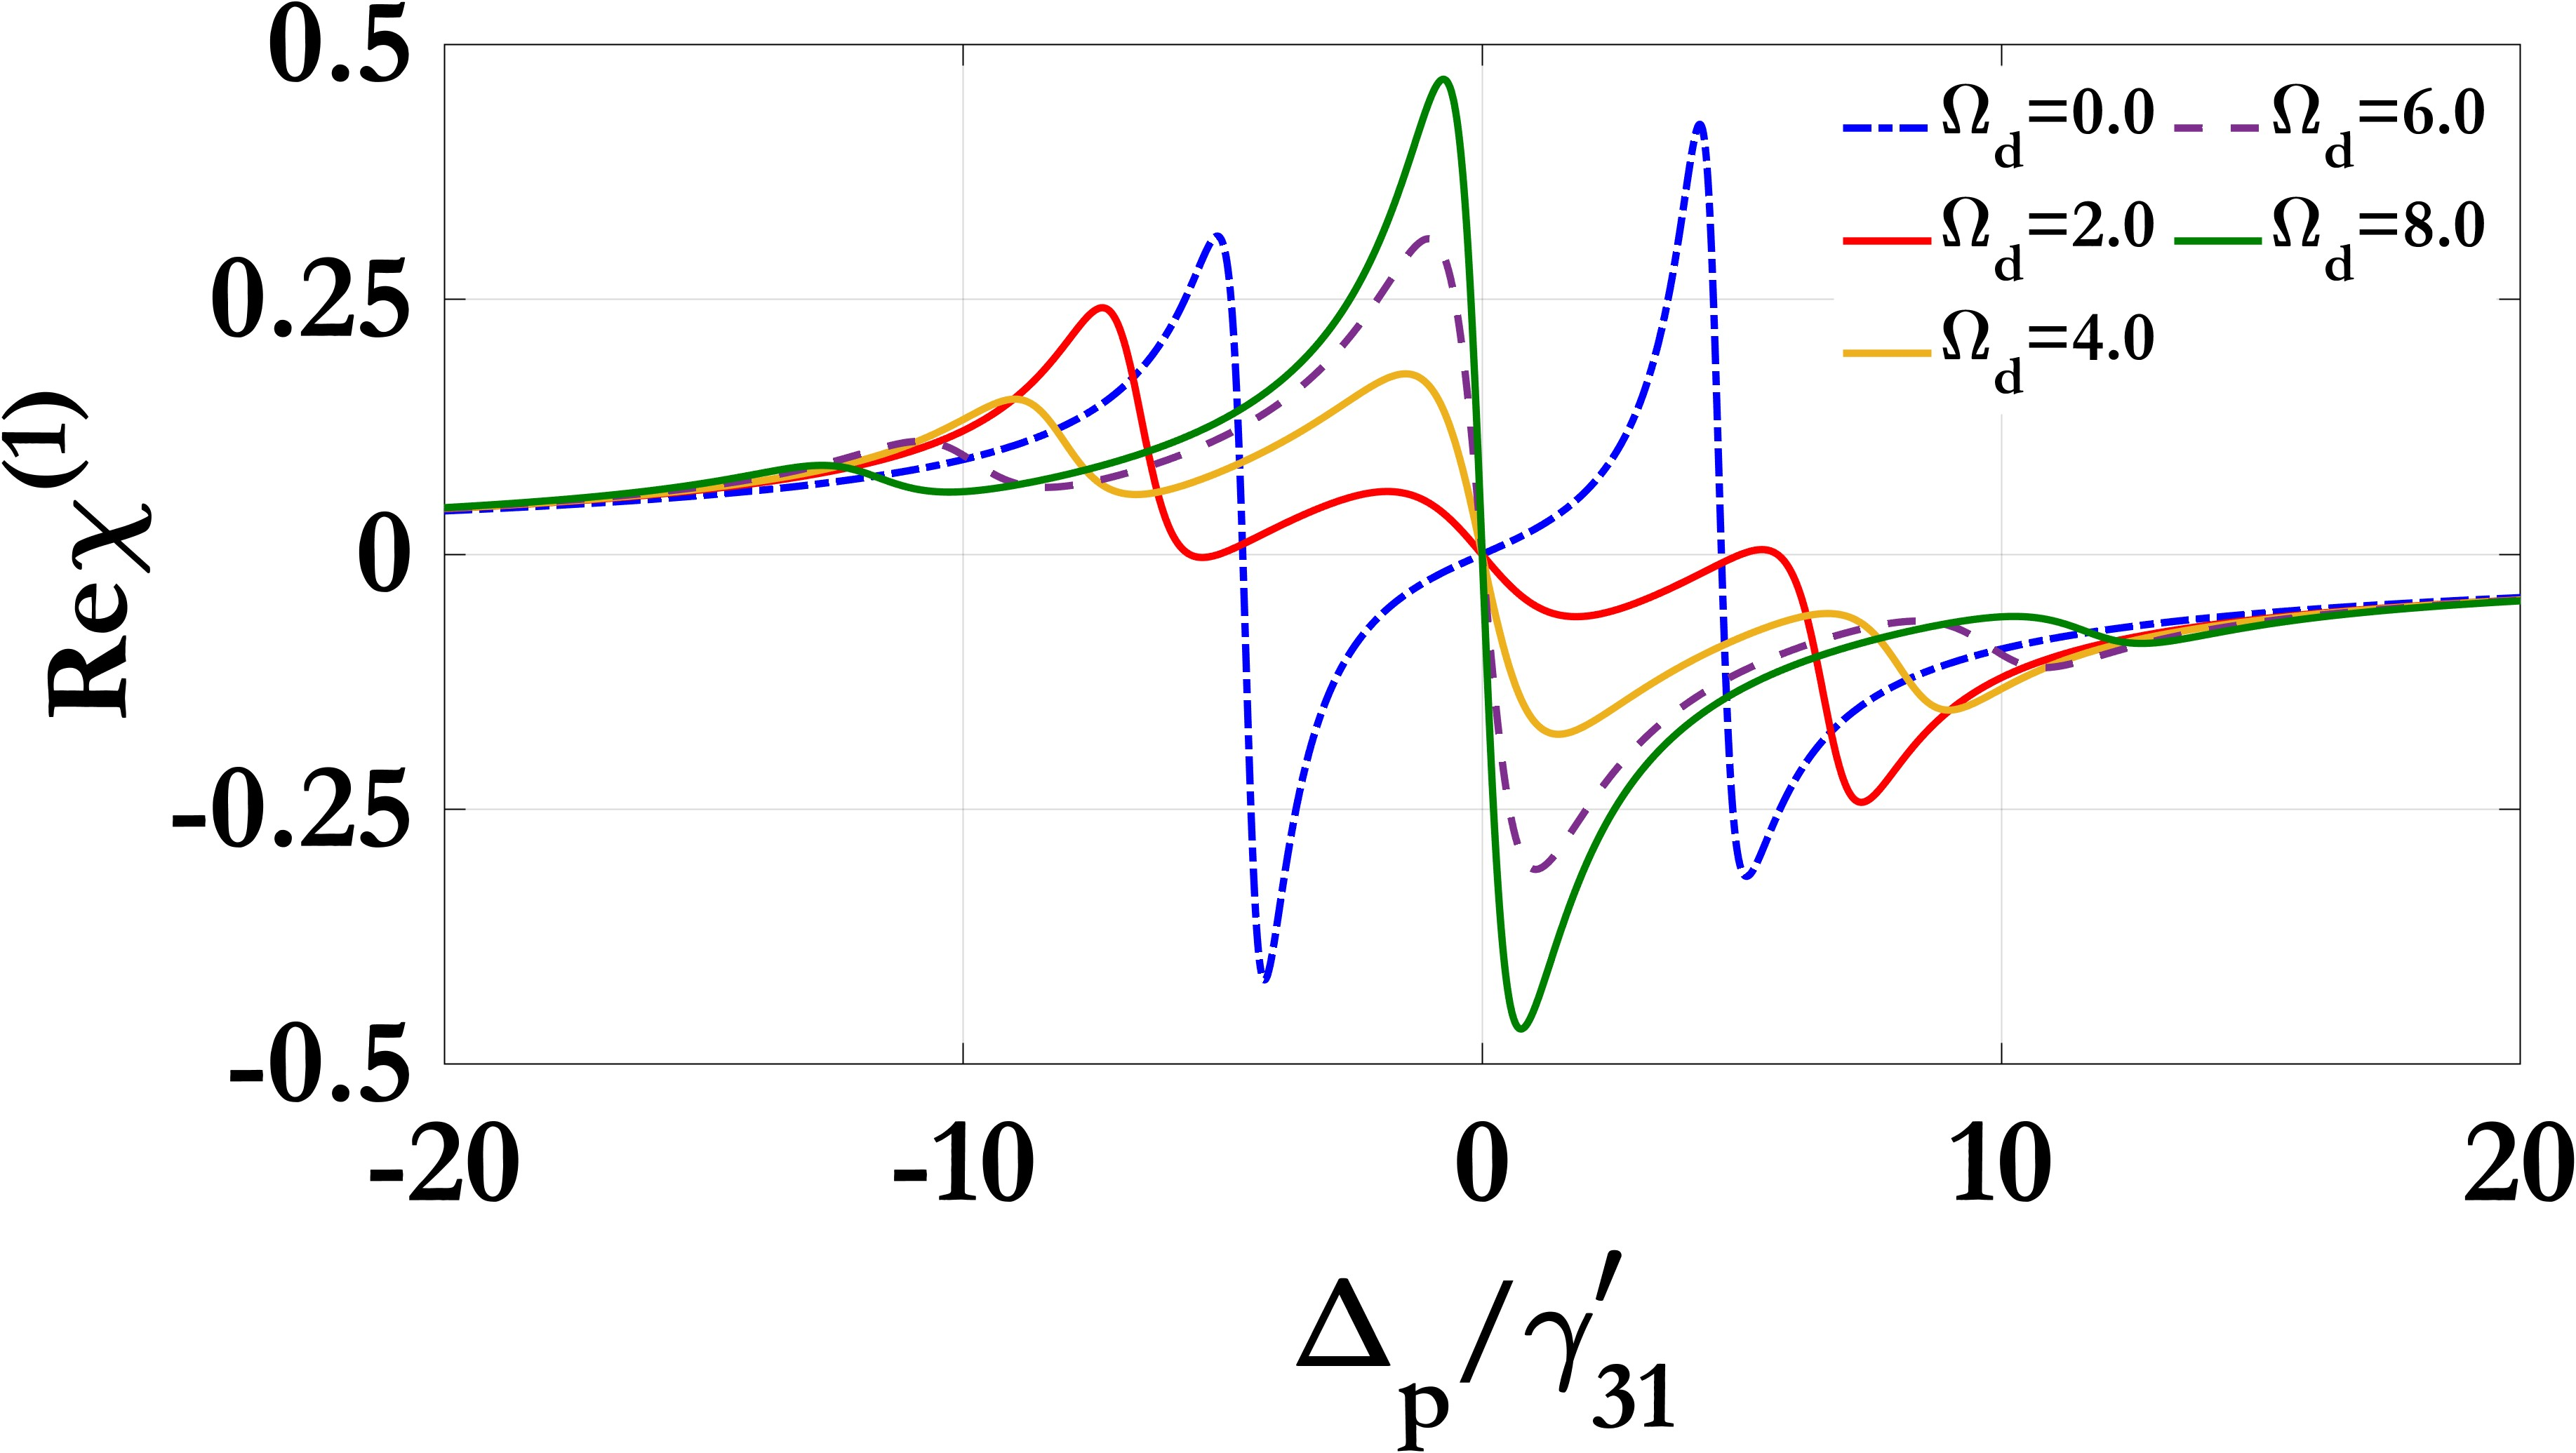
\includegraphics[width=\linewidth]{Assets/Real_chi1_Omega_d.jpeg}
      \subcaption{}
    \end{minipage}\label{fig:chi1_d}
   \end{figure}
   \begin{itemize}
    \item $\Omega_d$ modifies absorption: transparency windows form.
    \item Side peaks grow $\Rightarrow$ indicative of coherent interference.
    \item Re $\chi^{(1)}$ slope changes $\Rightarrow$ group velocity control.
  \end{itemize}
\end{frame}

\begin{frame}{Kerr Nonlinearity: Re $\chi^{(3)}$}
  \vspace{-4pt}
  \hspace*{43pt}
  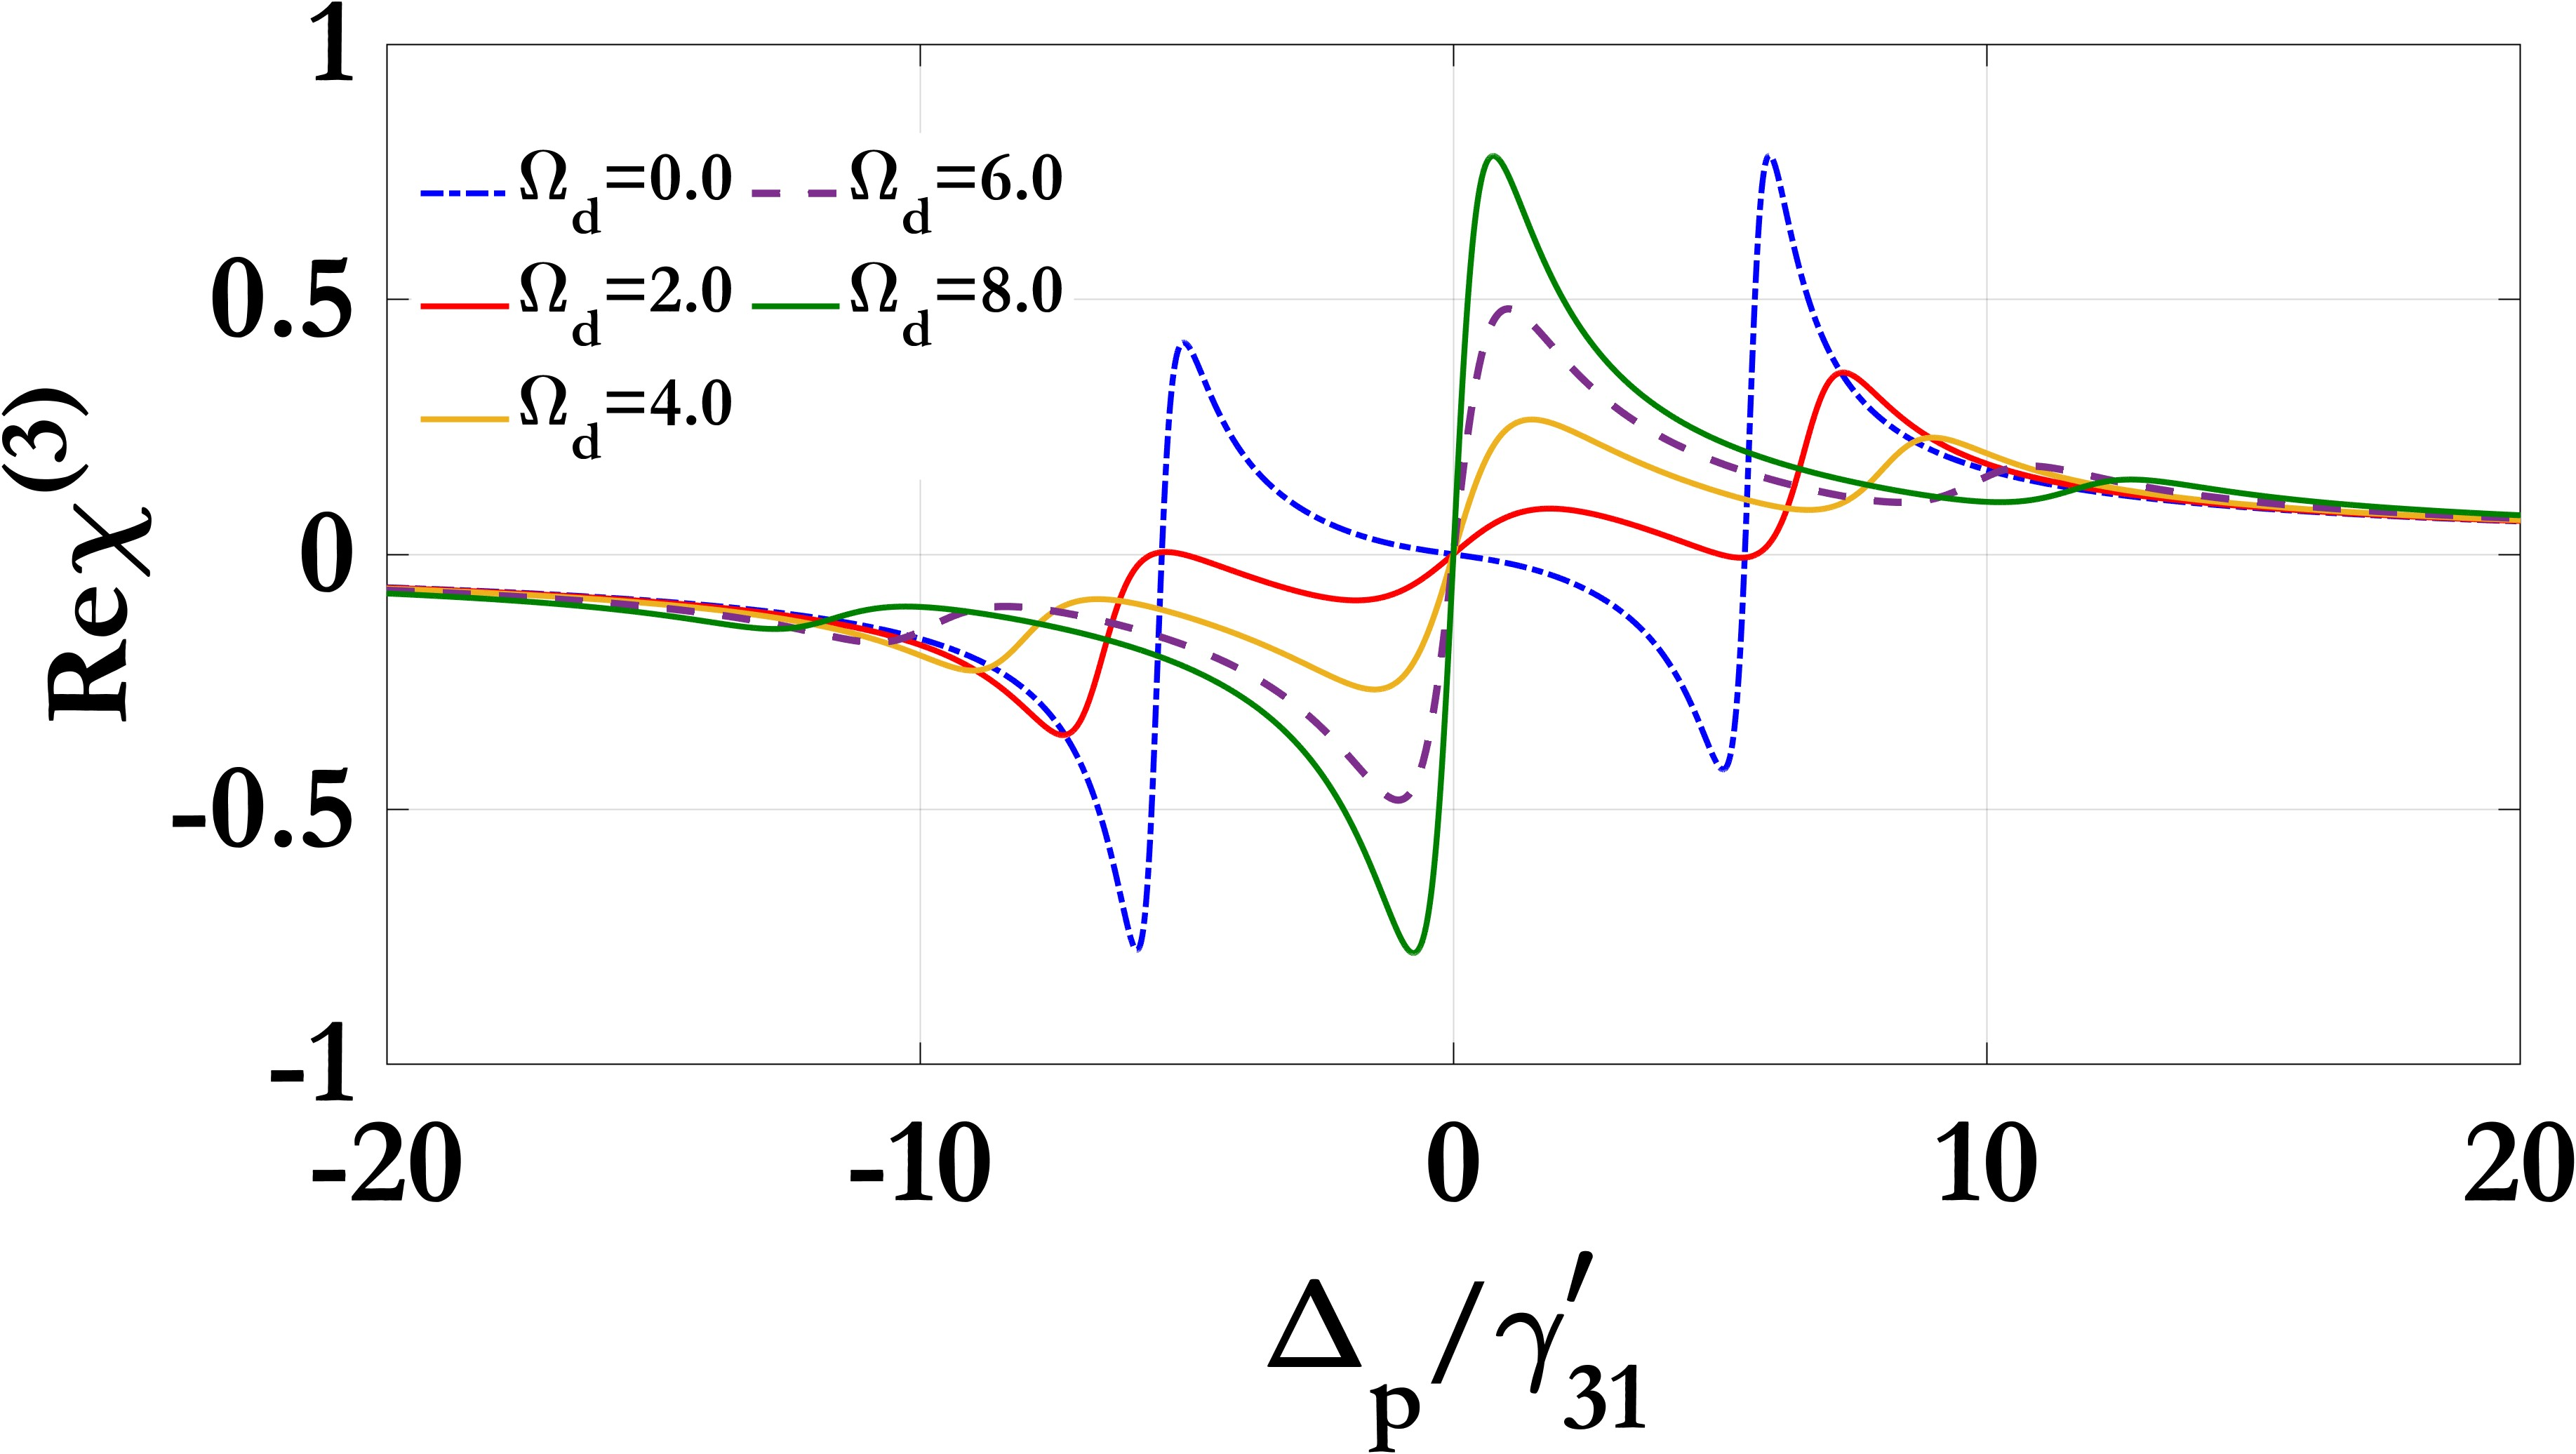
\includegraphics[width=0.75\textwidth]{Assets/Real_chi3_Omega_d.jpeg}
  \begin{itemize}
    \item $\Omega_c$, $\Omega_d$ enhance Kerr nonlinearity.
    \item $\chi^{(3)}$ control $\Rightarrow$ quantum gates, optical switches.
  \end{itemize}
\end{frame}

\begin{frame}{Modulation Instability Gain}
  \hspace*{45pt}
  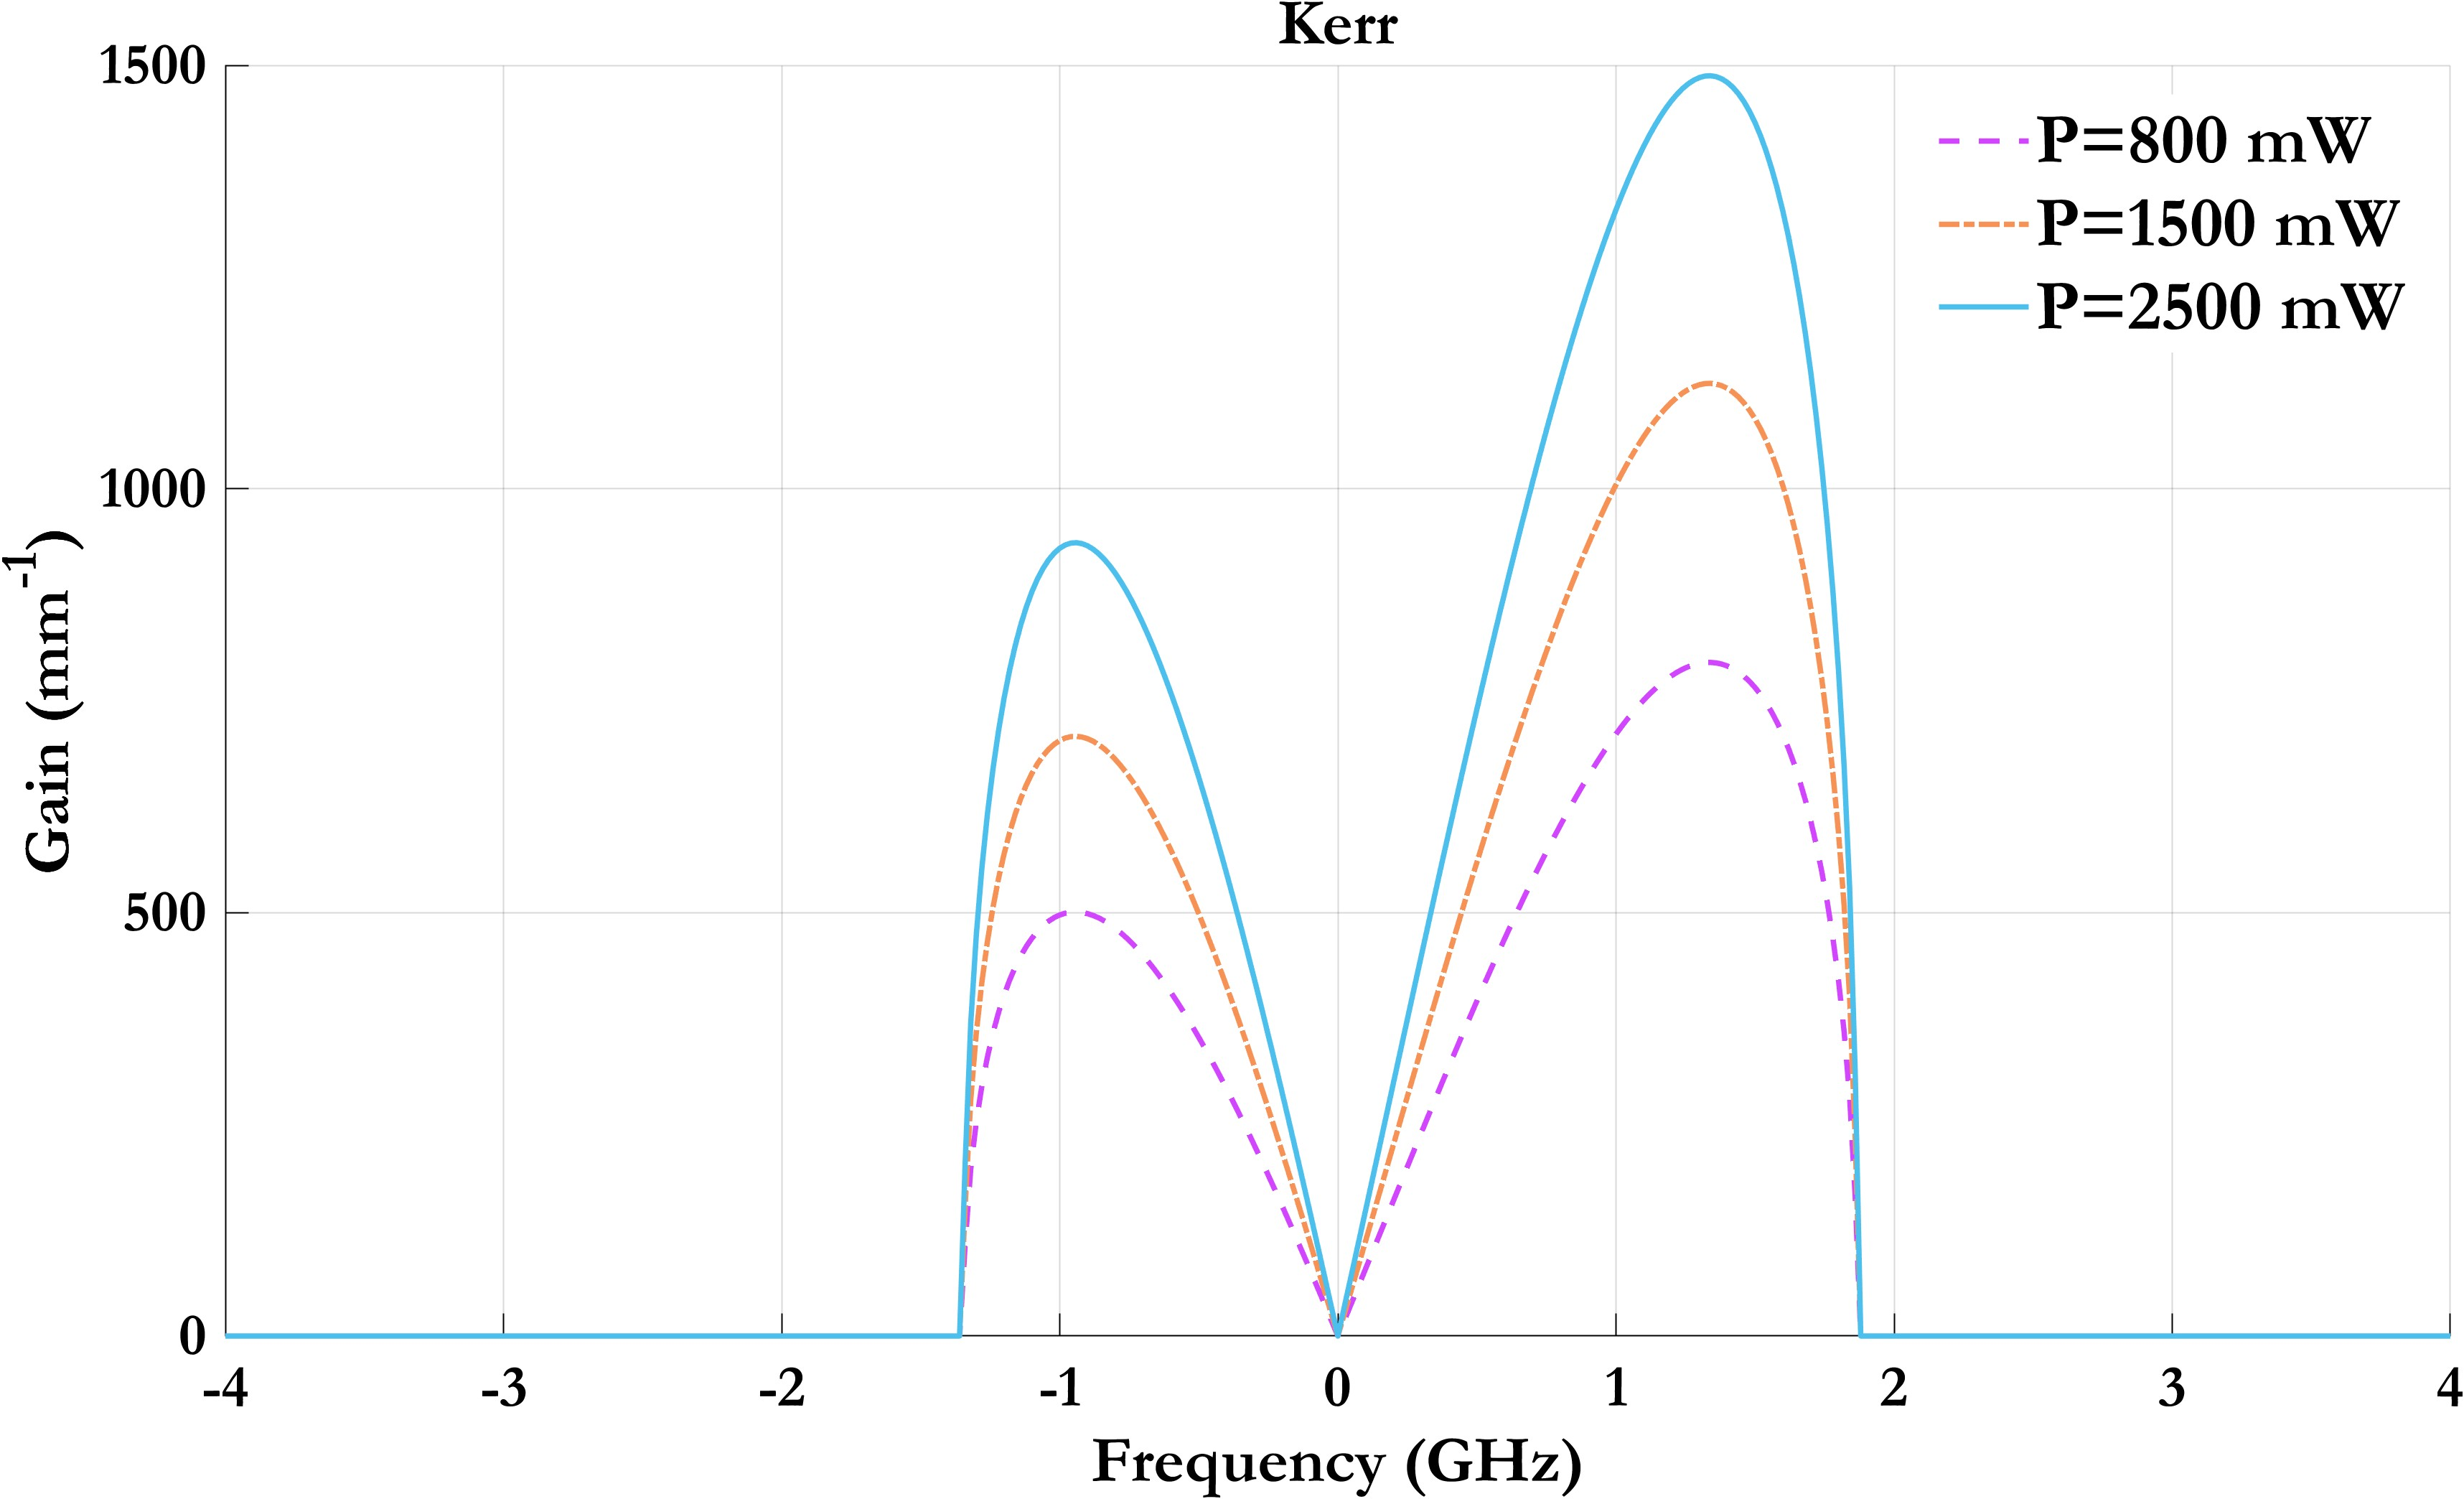
\includegraphics[width=0.69\textwidth]{Assets/G_v_Power.jpeg}
  \begin{itemize}
    \item MI gain shows symmetric sidebands $\Rightarrow$ phase matching.
    \item Gain increases with laser power.
    \item Peaks shift outward with higher nonlinear refractive index.
  \end{itemize}
\end{frame}

\begin{frame}{MI Gain}
  \vspace{-12pt}
  \hspace*{40pt}
  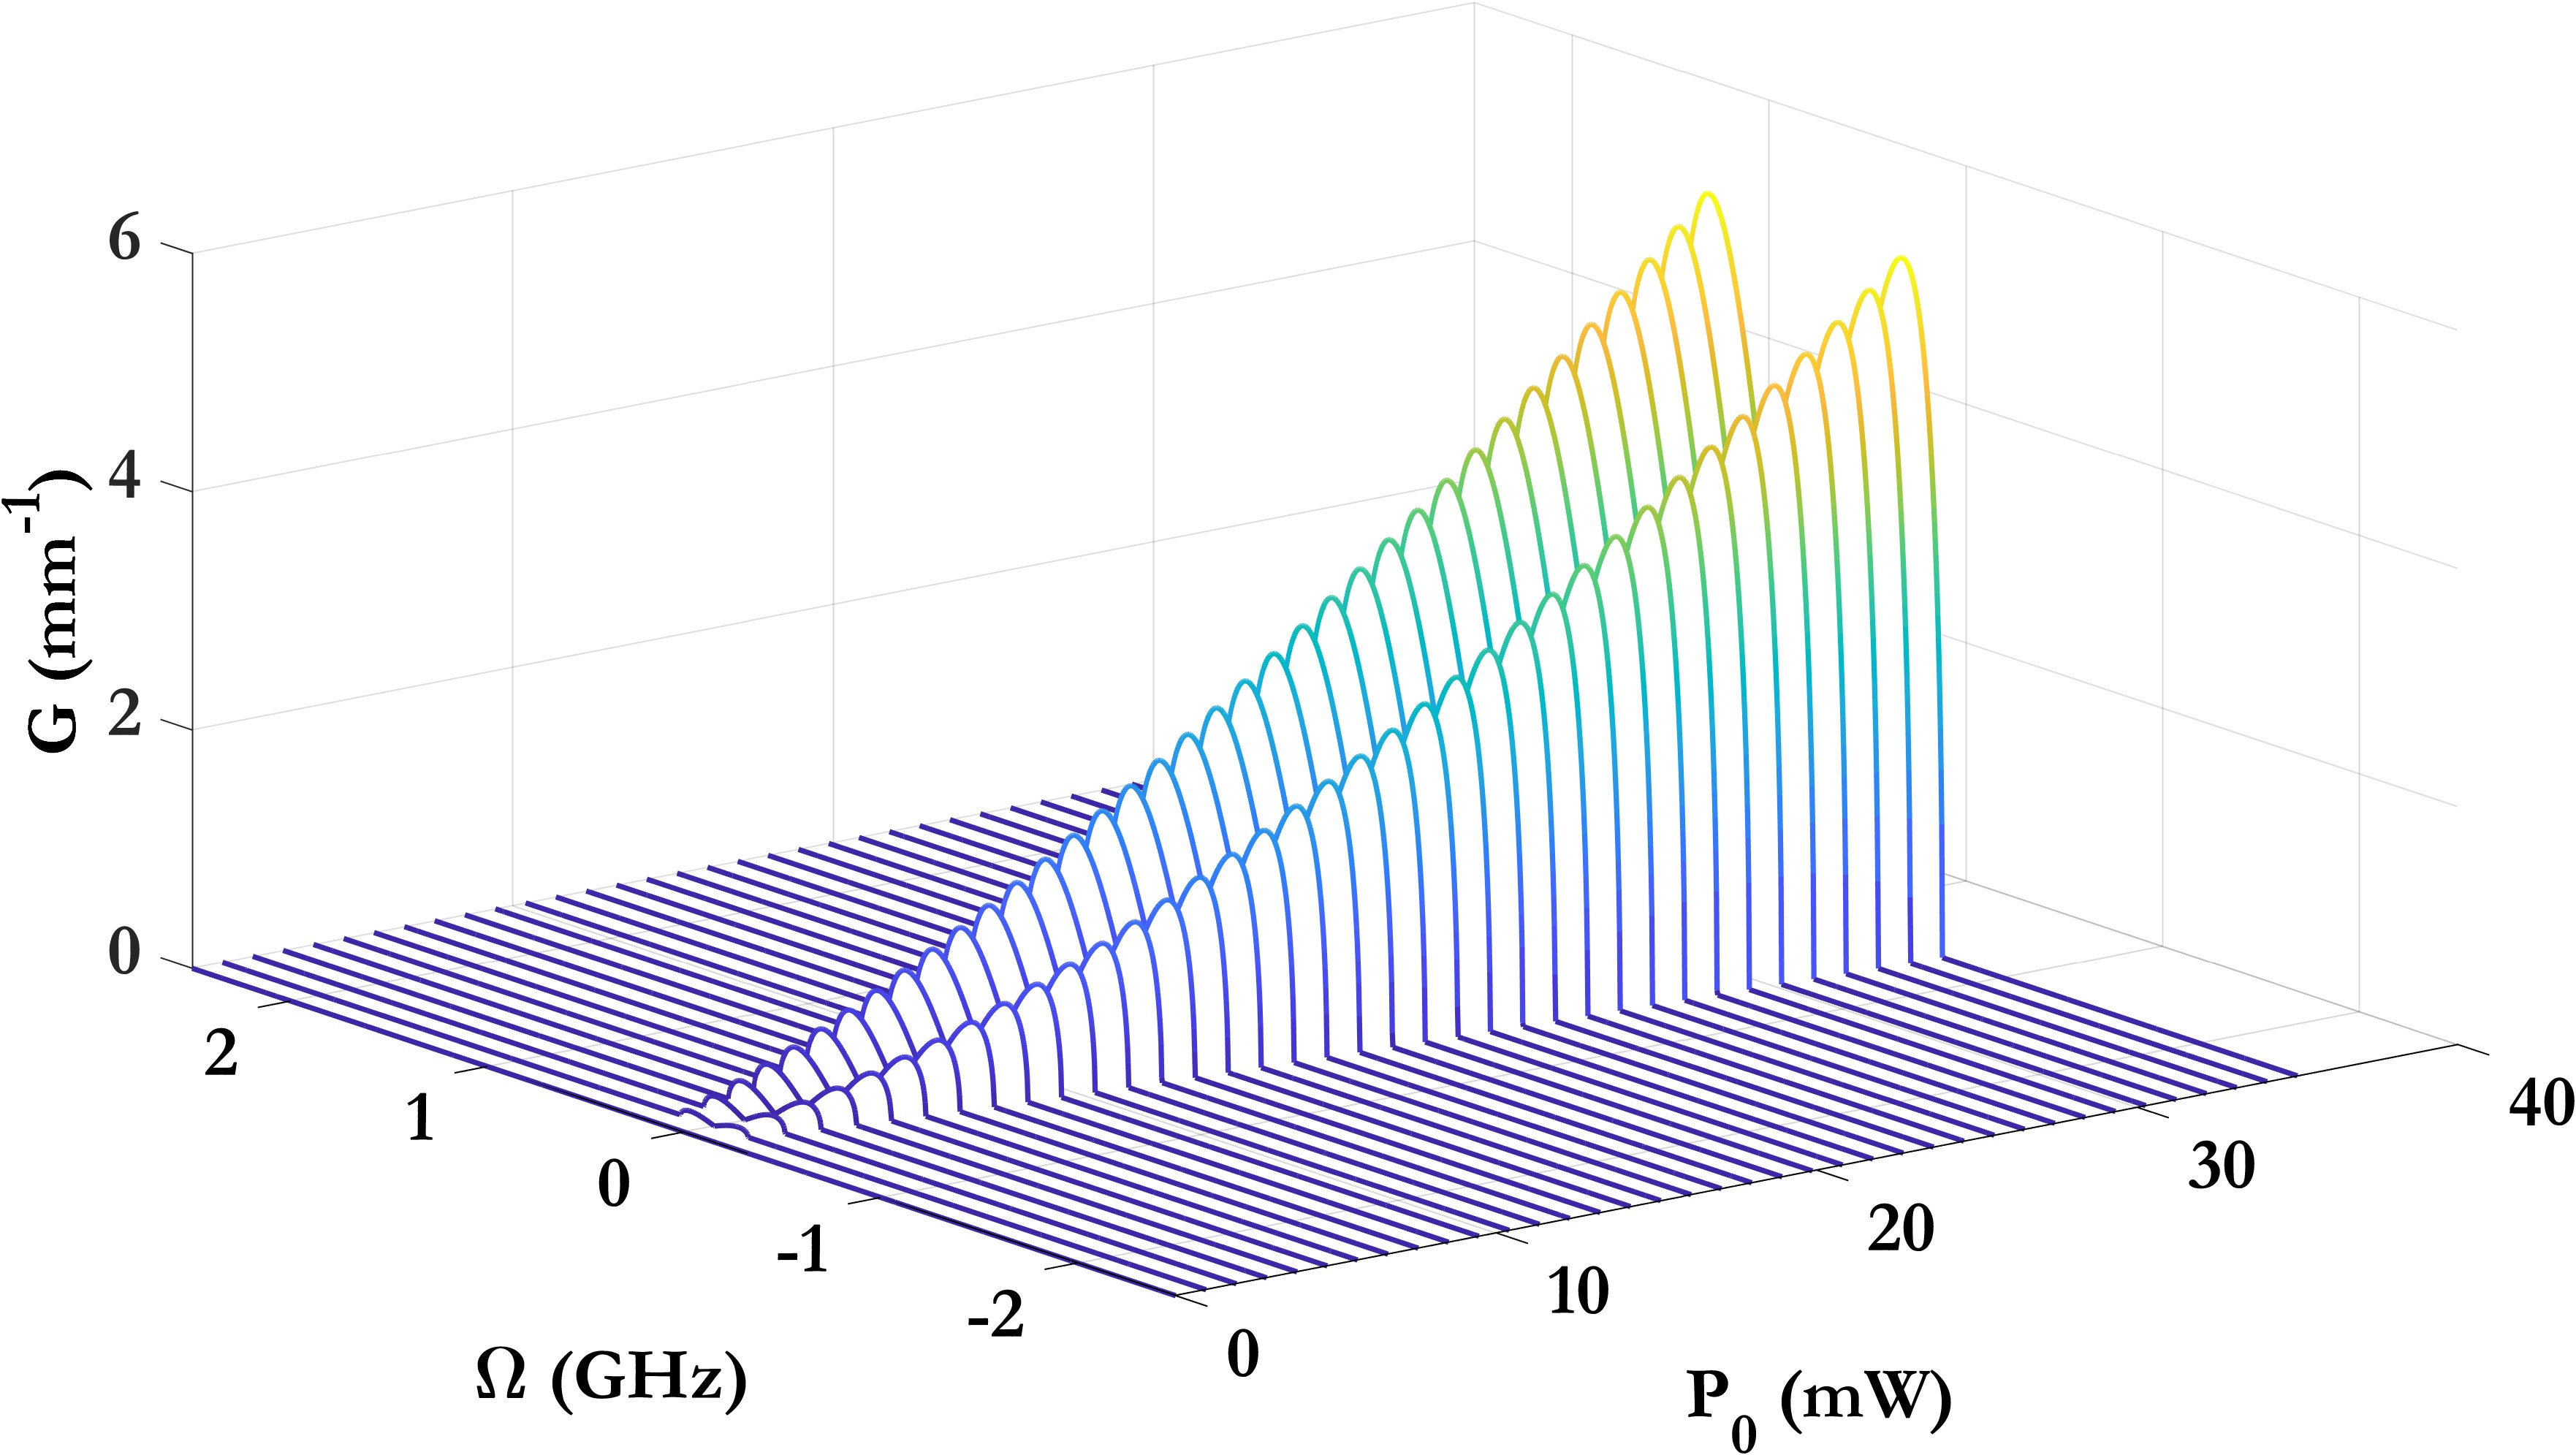
\includegraphics[width=0.8\textwidth]{Assets/Beta2_Kerr.jpeg}
  \begin{itemize}
    \item Fourth-order dispersion ($\beta_4$) broadens bandwidth.
  \end{itemize}
\end{frame}

\begin{frame}{Conclusion \& Applications}
  \begin{itemize}
    \item SQDs exhibit tunable nonlinearity through coherent control.
    \item Applications:
    \item Quantum memory and communication
    \item Slow light and optical buffers
    \item Frequency combs and all-optical logic
  \end{itemize}
\end{frame}

\begin{frame}{Questions}
  \centering
  {\Huge \bfseries Thank You For Your Attention}
\end{frame}

\end{document}